\documentclass{beamer}
\usepackage[utf8]{inputenc}
\usepackage{amsmath, amssymb, bm}
\usepackage{graphicx}
\usepackage{tikz}

\title{M\'etodos Estoc\'asticos em Otimiza\c{c}\~ao Cont\'inua}
\author{Danilo R. Souza}
\institute{Grupo de Otimiza\c{c}\~ao Cont\'inua - Unicamp}
\date{Abril de 2025}

\begin{document}

\frame{\titlepage}

\begin{frame}{Roteiro da Apresenta\c{c}\~ao}
\tableofcontents
\end{frame}

% --------------------------
\section{Motiva\c{c}\~ao e Contexto}
% --------------------------

\begin{frame}{Motiva\c{c}\~ao}
\begin{itemize}
    \item Problemas de otimiza\c{c}\~ao com dados massivos s\~ao cada vez mais comuns.
    \item Algoritmos determin\'isticos possuem custo computacional alto.
    \item Solu\c{c}\~oes estoc\'asticas s\~ao mais escal\'aveis.
\end{itemize}
\end{frame}

\begin{frame}{Exemplos de Aplica\c{c}\~oes}
\begin{itemize}
    \item Aprendizado de m\'aquina (deep learning)
    \item Vis\~ao computacional
    \item Processamento de sinais
    \item Invers\~ao de forma de onda (FWI)
\end{itemize}
\end{frame}

% --------------------------
\section{Formula\c{c}\~ao do Problema}
% --------------------------

\begin{frame}{Problema de Otimiza\c{c}\~ao Emp\'irica}
Queremos resolver:
\[
    \min_{x \in \mathbb{R}^d} f(x) = \frac{1}{n} \sum_{i=1}^n f_i(x)
\]
Onde cada \( f_i(x) \) representa a perda sobre um dado.
\end{frame}

\begin{frame}{Gradiente Padr\~ao (Determin\'istico)}
\[
    x_{k+1} = x_k - \eta \nabla f(x_k) = x_k - \eta \cdot \frac{1}{n} \sum_{i=1}^n \nabla f_i(x_k)
\]
\begin{itemize}
    \item Custo por itera\c{c}\~ao: \( O(n) \)
    \item Invi\'avel para grandes \( n \)
\end{itemize}
\end{frame}

% --------------------------
\section{Gradiente Estoc\'astico}
% --------------------------

\begin{frame}{Gradiente Estoc\'astico (SGD)}
\[
    x_{k+1} = x_k - \eta \nabla f_{i_k}(x_k)
\]
\begin{itemize}
    \item Escolhemos \( i_k \sim \mathcal{U}(\{1, \ldots, n\}) \)
    \item Reduz custo para \( O(1) \) por itera\c{c}\~ao
    \item Introduz vari\^ancia
\end{itemize}
\end{frame}

\begin{frame}{Mini-Batch SGD}
\[
    x_{k+1} = x_k - \eta \cdot \frac{1}{b} \sum_{i \in \mathcal{B}_k} \nabla f_i(x_k)
\]
\begin{itemize}
    \item \( \mathcal{B}_k \subset \{1, \ldots, n\},\quad |\mathcal{B}_k| = b \)
    \item Compromisso entre custo e vari\^ancia
\end{itemize}
\end{frame}

\begin{frame}{Figura: Converg\^encia}
\begin{center}
    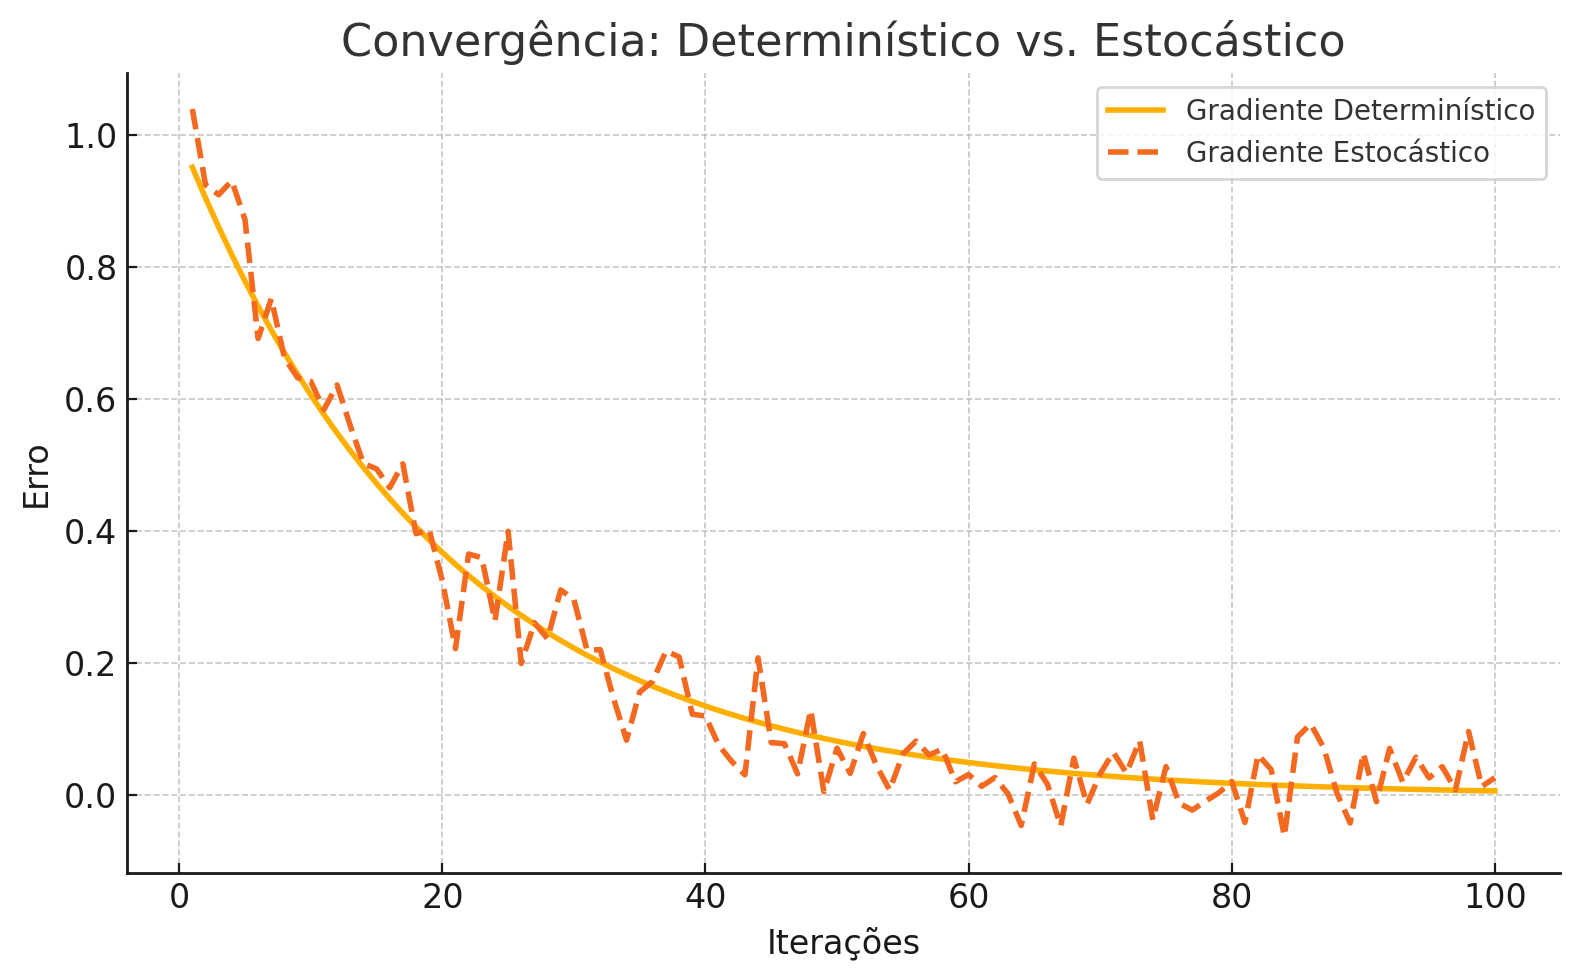
\includegraphics[width=0.8\textwidth]{convergencia_deterministico_estocastico.png}
\end{center}
\end{frame}

% --------------------------
\section{Aspectos Te\'oricos}
% --------------------------

\begin{frame}{Condi\c{c}\~oes para Converg\^encia}
\begin{itemize}
    \item Taxas de aprendizado devem satisfazer:
    \[
        \sum_{k=1}^\infty \eta_k = \infty, \qquad \sum_{k=1}^\infty \eta_k^2 < \infty
    \]
    \item Exemplo: \( \eta_k = \frac{1}{k} \)
\end{itemize}
\end{frame}

\begin{frame}{Vantagens e Desvantagens do SGD}
\begin{itemize}
    \item Vantagens:
    \begin{itemize}
        \item Alta escalabilidade
        \item Baixo custo por itera\c{c}\~ao
    \end{itemize}
    \item Desvantagens:
    \begin{itemize}
        \item Alta vari\^ancia
        \item Converg\^encia lenta e oscilat\'oria
    \end{itemize}
\end{itemize}
\end{frame}

% --------------------------
\section{Varia\c{c}\~oes e Extens\~oes}
% --------------------------

\begin{frame}{SGD com Momentum}
\[
    v_{k+1} = \mu v_k - \eta \nabla f_{i_k}(x_k), \quad x_{k+1} = x_k + v_{k+1}
\]
\begin{itemize}
    \item Suaviza oscila\c{c}\~oes
    \item Ajuda em vale estreitos
\end{itemize}
\end{frame}

\begin{frame}{Algoritmos Adaptativos}
\begin{itemize}
    \item AdaGrad
    \item RMSProp
    \item Adam
\end{itemize}
\end{frame}

\begin{frame}{Figura: Atualiza\c{c}\~oes com Momentum}
\begin{center}
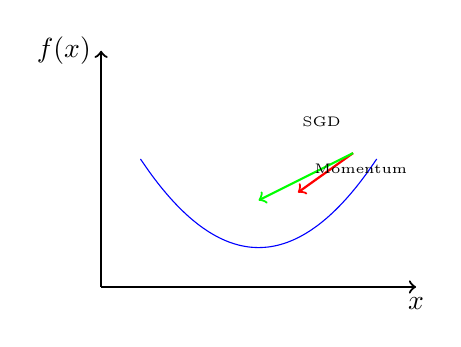
\begin{tikzpicture}
    \draw[->, thick] (0,0) -- (4,0) node[below]{$x$};
    \draw[->, thick] (0,0) -- (0,3) node[left]{$f(x)$};
    \draw[domain=0.5:3.5,smooth,variable=\x,blue] plot ({\x},{0.5*(\x-2)^2 + 0.5});
    \draw[->,red,thick] (3.2,1.7) -- (2.5,1.2);
    \node at (2.8,2.1) {\tiny SGD};
    \draw[->,green,thick] (3.2,1.7) -- (2.0,1.1);
    \node at (3.3,1.5) {\tiny Momentum};
\end{tikzpicture}
\end{center}
\end{frame}

% --------------------------
\section{Discuss\~ao e Aplica\c{c}\~oes}
% --------------------------

\begin{frame}{Quando Usar SGD?}
\begin{itemize}
    \item Bases de dados grandes
    \item Modelos com muitos par\^ametros
    \item Necessidade de solu\c{c}\~oes aproximadas r\'apidas
\end{itemize}
\end{frame}

\begin{frame}{Estudo de Caso: FWI}
\begin{itemize}
    \item Fun\c{c}\~ao objetivo altamente n\~ao convexa
    \item Simula\c{c}\~oes caras
    \item SGD pode reduzir custo computacional com boa regulariza\c{c}\~ao
\end{itemize}
\end{frame}

% --------------------------
\section{Resumo e Encerramento}
% --------------------------

\begin{frame}{Resumo da Apresenta\c{c}\~ao}
\begin{itemize}
    \item Motivamos o uso de m\'etodos estoc\'asticos
    \item Apresentamos SGD e varia\c{c}\~oes
    \item Discutimos vantagens, limita\c{c}\~oes e aplica\c{c}\~oes
\end{itemize}
\end{frame}

\begin{frame}{Refer\^encias}
\small
\begin{itemize}
    \item Bottou, L. et al. (2018). Optimization Methods for Large-Scale Machine Learning.
    \item Bubeck, S. (2015). Convex Optimization: Algorithms and Complexity.
    \item Ruder, S. (2016). An overview of gradient descent optimization algorithms.
\end{itemize}
\end{frame}

\begin{frame}{Obrigado!}
\centering
D\'uvidas? Coment\'arios? Sugest\~oes?
\end{frame}

\end{document}
